\documentclass[11pt]{article}
\usepackage[a4paper, total={170mm,257mm}, left=20mm, top=20mm]{geometry}
\usepackage{graphicx}
\usepackage{booktabs}
\usepackage{amsmath}
\usepackage{amssymb}
\usepackage{float}
\usepackage[style=authoryear, backend=biber, maxcitenames=2]{biblatex}
\DeclareDelimFormat{nameyeardelim}{\addcomma\space}
\usepackage{xcolor}
\usepackage{hyperref}

\newcommand{\atiyab}[1]{\textcolor{teal}{\textbf{[Atiyab: #1]}}}
\newcommand{\fausto}[1]{\textcolor{blue}{\textbf{[Fausto: #1]}}}
\newcommand{\juan}[1]{\textcolor{purple}{\textbf{[Juan: #1]}}}
\newcommand{\todo}[1]{\textcolor{red}{\textbf{[TODO: #1]}}}
\newcommand{\placeholder}[1]{\fbox{\parbox[c][4cm][c]{0.8\linewidth}{\centering\small\textit{Figure to come.} #1}}}

\addbibresource{refs.bib}

% Alternative title that states the finding (10 words, no punctuation):
% How network structure allocates performance in collective problem solving
\title{The impact of network structure on distributed problem solving}
\author{Fausto Gernone \and Atiyab Zafar \and Juan G.\ Restrepo}
\date{Draft, 30 September 2026\\ \small for npj Complexity, collection ``Decision-making in Structured Groups''}

\begin{document}
\maketitle


\begin{abstract}
    The foundamental challenge faced by any organisation is how to solve problems when knowledge is imperfect and dispersed across members. We ask how communication structure shapes this process. We study a model where agents on a directed communication network individually face the same constraint-satisfaction problem whose constraints are replaced over time. They learn by testing constraints and exchanging beliefs with their neighbours. The communication rate is normalised so that the average agent receives one message per period on every network. \todo{short run behaviour} In the long run, average performance is unrelated to network structure. However, relative individual performance within a network rises with in-degree along a single curve that all topologies share. In other words, communication structure has no effect on how well the organsiation performs on average, but it allows to allocate relative performance. A mean-field argument accounts for both regularities.
\end{abstract}


%======================================================================
\section{Introduction}\label{sec:intro}
%======================================================================

Problem-solving under uncertainty is a foundamental challenge for any organization. In practice, individuals solve problems and take decisions udner conditions of incomplete knowledge and bounded rationality. Moreover, knowledge is typically scattered across group members and can become outdated while it is being used. A foraging group tracks food patches that appear and disappear, and different engineers in a software firm might speialise in different parts of the code. In each case the members hold different pieces of the problem, pass some of those pieces on, and act on what they have. Who can learn from whom depends on the structure of the organization, which is sometimes a product of the group's history and sometimes a design choice. This paper investigates how the structure of that network affects the quality of decisions, both for the group as a whole and for its individual members.

Different fields have answered the question differently. Organisation theory treats hierarchy as a response to bounded rationality and to the cost of processing information: concentrating problem-solving in a few well-connected positions reduces the communication a group needs \parencite{simon1962architecture, radner1993organization, bolton1994firm}. Work on collective problem solving in networks finds a trade-off instead. Well-connected groups spread good solutions quickly but may settle on them too early, while sparser groups preserve the variety of partial solutions that a hard problem eventually needs \parencite{lazer2007network, mason2008propagation, fang2010balancing}, and whether the trade-off appears depends on the task and on how members copy one another \parencite{shore2015facts, barkoczi2016social}. Models of opinion dynamics and social learning ask when interaction on a network produces agreement, and when it produces accuracy \parencite{bala1998learning, jackson2011overview, noorazar2020classical}. The two can favour different structures: \textcite{berekmeri2020optimal} find that agreement is highest in egalitarian networks, while accuracy can be highest in hierarchical ones in which a few members specialise in gathering information. 

Recent contributions to this collection push the question beyond pairwise structure, and beyond structure itself. \textcite{hebert2025governance} model governance as a satisfiability problem in which a population must make many interdependent decisions, and represent who deliberates with whom as a hypergraph of overlapping groups; small overlapping groups turn out to deliver coherent decisions at low coordination cost. \textcite{marchpons2026symmetry} show that a group choosing among equally good options can deadlock under pairwise influence alone, and that interactions within larger groups are what break the tie. \textcite{garg2026synergy} argue that structure acts on performance through the way information is processed, and that the balance between local redundancy and long-range synergy predicts group performance better than structure does. Observational work on real teams points the same way: in escape rooms, effective teams coordinate throughout and share participation evenly, and no single arrangement is best for every task \parencite{oszabo2026coordination}. The common thread is that structure matters through the information it moves. We take that idea to its end by holding the amount of information moved fixed, and asking what structure still does.

In our model, agents face a hidden set of logical constraints on $K$ binary choices, which determine which combinations of choices are feasible, and every agent choose a full combination. Agents learn about the constraints through testing and communication. They test whether candidate constraints hold and re-test their existing beliefs, remembering when a previously believed constraint is found to be false. They also receive beliefs from their neighbours: each neighbour shares its most recently updated belief that the receiving agent either lacks or disagrees with. When an agent acquires a positive belief about a constraint, it adjusts its choices to reduce violations of the constraints it currently believes hold. The environment changes over time as constraints are retired and replaced, so previously correct beliefs can become outdated and spread through communication.

\todo{short-run finding, one or two sentences, once the runs are in.} Here we show that in the long run, average performance is statistically indistinguishable across random, small-world, scale-free and layered networks of equal mean in-degree, and across mean in-degrees from about 4 to 50. Position within a network matters a great deal. An agent's long-run performance improves with the number of others it hears from, and at a given in-degree it is the same in every topology: the relation is a single curve that all networks share. What structure decides is which points on that curve are occupied. A scale-free network creates a few positions with very high intake, and the agents in them outperform the periphery by 3 to 5 violations out of 60 constraints. The reason is simple once intake is written down. Normalisation fixes each network's mean intake at one message per period, so structure can move average performance only through the spread of intake around that mean, which is a second-order effect, while it moves the spread of performance directly. Centralisation therefore leaves the group average almost unchanged and gives a designer the choice of who its best-informed members will be.


%======================================================================
\section{Methods}\label{sec:methods}
%======================================================================

\subsection{Entities and state}

The model has $N$ agents who work on the same problem: choosing values for $K$ binary variables so as to satisfy a set of constraints that none of them can see directly. Agents sit on the nodes of a fixed directed graph $G$. An edge $j \to i$ means that agent $i$ can receive information from agent $j$. We call $j$ an in-neighbour of $i$, write $k_i$ for the in-degree of $i$, and write $\langle k\rangle$ for the mean in-degree, which equals the mean out-degree.

\paragraph{Decision variables.} Each agent holds a private assignment $x^{(i)} \in \{0,1\}^K$. Agents never exchange assignments. What they exchange are beliefs about the constraints.

\paragraph{Constraints.} The environment scores assignments against a set $\mathcal{C}$ of $M = \alpha K$ clauses. Each clause involves two distinct variables and one of two operators. An \textsc{and} clause on $(x_a, x_b)$ is satisfied when $x_a = x_b = 1$; an \textsc{xor} clause is satisfied when exactly one of the two equals 1. The universe $\mathcal{U}$ of possible clauses therefore has $2\binom{K}{2} = K(K-1)$ elements, 870 at $K = 30$. Clauses enter $\mathcal{C}$ as independent draws from $\mathcal{U}$, so $\mathcal{C}$ is a multiset: at $M = 60$ a given slot coincides with another one in about 7\% of cases.

\paragraph{Performance.} Agent $i$'s violation count $V_i$ is the number of slots of $\mathcal{C}$ that $x^{(i)}$ violates; lower is better. We track the population average $\bar V$ and the best agent's count $V_{\min}$. Homogeneity,
\[
H = \frac{1}{K} \sum_{j=1}^{K} \frac{\max(n_j,\, N-n_j)}{N},
\]
where $n_j$ is the number of agents with $x_j = 1$, measures how far agents agree on each variable, and runs from $1/2$ to 1. Agents never observe $\mathcal{C}$ or their own $V_i$. They see only the outcomes of their own tests and the beliefs their neighbours send them.

\paragraph{Beliefs.} Agent $i$ holds a store $\mathcal{B}_i \subseteq \mathcal{U}$ of signed beliefs. A positive belief, $\sigma_i(c) = +1$, says that clause $c$ is currently a constraint. A negative belief, $\sigma_i(c) = -1$, says that it is not. Only positive beliefs guide the agent's assignment. Negative beliefs matter in two other ways: they stop an agent from re-adopting a clause it has found to be false, and they can be passed on. The store is kept in recency order, from the belief touched longest ago to the one touched most recently, where a belief counts as touched when it is adopted, tested or received. It holds at most $2M$ beliefs. When an addition takes it over that limit, the least recently touched belief is evicted, whatever its sign.

A positive belief about a clause that is no longer in $\mathcal{C}$ is \emph{stale}. Stale beliefs are the model's misinformation. To the agent holding one, it looks exactly like knowledge.

\subsection{Initialisation}

Every assignment is drawn uniformly at random, one fair coin per variable, and every belief store starts empty. The $M$ clauses of $\mathcal{C}$ are drawn independently: first the operator, each with probability $1/2$, then a pair of distinct variables uniformly at random. The network is generated as described below, and the link firing probability $s = 1/\langle k\rangle$ is computed once from its mean in-degree.

\subsection{Per-period dynamics}

Time runs in discrete periods. In each period the agents act one at a time, in an order reshuffled every period, and the environment changes once they have all acted. Updating is asynchronous, so an agent that acts late in a period can receive a belief that another agent acquired earlier in the same period. Tests are scored against $\mathcal{C}$ as it stands at the start of the period. Each agent's turn has four steps.

\paragraph{1. Test.} With probability $1/2$ the agent tests a new clause. It draws a candidate uniformly from $\mathcal{U}$ and, if it already holds a belief about the candidate, draws again, up to ten times. If the final candidate is unheld and belongs to $\mathcal{C}$, the agent adopts it as a positive belief. Otherwise the candidate is discarded without a record, so agents do not accumulate negative beliefs about clauses they never held. With at most 120 beliefs in a universe of 870, the chance that all eleven draws hit held beliefs is below $10^{-9}$, so in effect the candidate is uniform over the clauses the agent has no belief about.

With probability $1/2$ the agent instead re-tests one of its beliefs, chosen uniformly from $\mathcal{B}_i$ whatever its sign, and sets it to the truth. A positive belief whose clause has left $\mathcal{C}$ becomes negative: the clause is falsified, and the agent remembers that it is. A negative belief whose clause is back in $\mathcal{C}$ becomes positive. A correct belief is confirmed. In each case the tested belief moves to the most recent end of the store.

\paragraph{2. Repair.} If the test produced a positive belief, new or restored, the agent revises its assignment around that clause. It takes the clause's two variables in random order and flips each one if and only if the flip strictly reduces the number of violated positive beliefs that contain that variable; ties are rejected. The variables are handled one after the other, so the decision on the second takes the first into account. Falsifying a belief triggers no repair. The agent stops trying to satisfy the clause but leaves its variables as they are.

\paragraph{3. Communicate.} The agent then goes through its in-neighbours. The link from each in-neighbour $j$ fires with probability $s$, independently across links and periods. When it fires, $j$ sends a single belief. Among the beliefs on which the two agents disagree, meaning those that $j$ holds and $i$ either lacks or holds with the opposite sign, it is the one $j$ touched most recently. Agent $i$ adopts $j$'s sign for that clause, adding the belief or overwriting its own, and the belief moves to the most recent end of $i$'s store. If $i$ already agrees with everything $j$ holds, nothing is sent. Sending leaves the sender unchanged. Messages carry beliefs and not the truth, so a stale positive travels as easily as a correct negative, and only tests check beliefs against the world.

Because $s = 1/\langle k\rangle$, agent $i$ expects
\begin{equation}\label{eq:intake}
\lambda_i = s\,k_i = \frac{k_i}{\langle k\rangle}
\end{equation}
firing links per period. The population average of $\lambda_i$ is exactly 1 on every network, whatever its structure or density, while individual intake still grows with in-degree. Slightly fewer than $\lambda_i$ beliefs actually arrive, because a link can fire when there is nothing to disagree about.

\paragraph{4. Repair again.} Whenever a received belief is positive and is either new to $i$ or overturns a negative belief of $i$, the agent repairs around it as in step 2. Repairs happen as beliefs arrive, so an agent with several firing links can repair several times in one period.

The capacity limit is applied after every change to the store in steps 1 and 3.

\subsection{Environmental change}

After every agent has acted, the environment drifts. In each period whose index is a multiple of $\tau$, one slot of $\mathcal{C}$, chosen uniformly, is overwritten by a fresh clause drawn as at initialisation. By default $\tau = 1$, one replacement per period. A given slot is hit with probability $1/M$ at each replacement, so a clause stays in $\mathcal{C}$ for $M\tau$ periods on average (60 at the default), and the whole set turns over on that time scale.

Retirement does not reach into agents' stores. Everyone who believed the retired clause now holds a stale belief, and keeps acting on it until a test or a message corrects it. The fresh clause can coincide with one retired earlier. When it does, stale beliefs about it become correct again, and negative beliefs about it become wrong. All statistics are computed after the replacement.

\subsection{Networks}

We use four standard generators, set to give a mean in-degree close to 4 at $N = 80$, and one designed family.

\emph{Random} (Erd\H{o}s-R\'enyi): every ordered pair of distinct agents $(j, i)$ is linked $j \to i$ independently with probability $0.05$, so in- and out-degree are independent.

\emph{Small world} (Watts-Strogatz): agents sit on a ring and each is linked to its four successors. Each of these links is given a random direction, and each directed link is then rewired with probability $0.1$ by keeping its source and moving its target to a random agent.

\emph{Scale free} (Barab\'asi-Albert): the network starts from four fully connected agents. Every further agent attaches to up to four existing agents, chosen with probability proportional to their current in-degree, and each new link is given a random direction. Orienting links after the structure is built makes in- and out-degree positively correlated here and negatively correlated in the small-world network. Because attachment follows in-degree, an agent whose own links all point outwards (roughly one agent in sixteen) never gains an in-link and never receives anything.

\emph{Layered}: agents are split at random into three near-equal layers. Each ordered pair within a layer is linked with probability $0.10$, and each ordered pair across layers with probability $0.03$. The network has layers but no hubs, and its degree distribution is close to that of the random network. \todo{settle the name: layered or hierarchical}

\emph{Uniform in-degree} (designed): each agent is assigned a target in-degree, and its in-neighbours are drawn uniformly without replacement from the other agents; out-degrees are left free. Three designs spread in-degrees evenly over 1-10 ($N = 100$, $\langle k\rangle = 5.5$), 1-50 ($N = 100$, $\langle k\rangle = 25.5$) and 1-100 ($N = 101$, $\langle k\rangle = 50$). When compared with these, the random and scale-free networks are also run at $N = 100$.

\subsection{Simulation protocol and statistics}

Table~\ref{tab:params} lists the defaults. Each run lasts $T = 2000$ periods, and long-run statistics are time averages over the last 500. An agent's long-run violation count is its mean over that window. Each seed draws a new network, new initial assignments and a new $\mathcal{C}$. The four-topology comparison uses ten seeds per topology and the designed networks eight, so topology comparisons are unpaired and report means and standard deviations across seeds.

For position effects we compute, in each run, the Spearman correlation between in-degree and long-run violations (tied ranks averaged), the gap in mean long-run violations between the eight agents with the highest in-degree and the eight with the lowest, and the in-degree percentile of the best-performing agent (mid-rank for ties). Pooled curves bin agents by in-degree and drop bins with fewer than five agents.

The model is written in Python with Mesa, NetworkX and NumPy. Parts of the implementation iterate over hashed objects, so Python's per-process hash randomisation changes the random stream; all runs fix \texttt{PYTHONHASHSEED}. \todo{state the value used; add the statistics and reproducibility paragraph the journal requires}

\begin{table}[H]
\centering
\caption{Default parameters.}
\label{tab:params}
\small
\begin{tabular}{@{}llr@{}}
\toprule
Symbol & Meaning & Value \\
\midrule
$N$ & agents & 80 (100-101 for designed networks) \\
$K$ & binary variables & 30 \\
$\alpha$ & clause density & 2 \\
$M = \alpha K$ & clauses in $\mathcal{C}$ & 60 \\
$|\mathcal{U}| = K(K-1)$ & possible clauses & 870 \\
$2M$ & belief-store capacity & 120 \\
$\tau$ & periods between clause replacements & 1 \\
$s = 1/\langle k\rangle$ & link firing probability & set by the network \\
 & test split, new clause against held belief & 1:1 \\
 & redraws when testing a new clause & up to 10 \\
$T$ & periods per run & 2000 \\
 & long-run averaging window & last 500 periods \\
 & seeds per condition & 10 (8 for designed networks) \\
\bottomrule
\end{tabular}
\end{table}


%======================================================================
\section{Results}\label{sec:results}
%======================================================================

\subsection{Simulations}

All runs use the model as specified in Methods, with $\tau = 1$, $T = 2000$, and long-run statistics averaged over the final 500 periods.

\subsubsection{Misinformation dynamics}

Because the environment keeps changing, part of what agents believe is always out of date. In earlier runs of this model at $\tau = 1$, around 40-50\% of positive beliefs were stale in the long run. \todo{confirm across seeds and topologies; figure below} Every retirement starts a small contest over the population. At the moment a clause is retired, everyone who believed it still does and nobody disbelieves it. Disbelief has to be produced by tests and then spread by messages, against believers who keep passing the clause on. In instrumented runs the two flows nearly cancel: early in a run we counted 98,610 corrections of a stale belief by a received negative against 92,727 re-infections of an agent that had already corrected it. \todo{measured at $\tau = 10$; re-measure at $\tau = 1$} Stale beliefs are removed by the small net difference, which comes from testing and from the recency rule. A disbelief is usually fresher than the belief it contradicts, so it gets sent first more often.

\begin{figure}[H]
\centering
\placeholder{Share of positive beliefs that are stale, over time, by topology (default model, mean over seeds). Possibly a second panel following one retired clause: share of agents believing and disbelieving it against time since retirement.}
\caption{Misinformation dynamics. \todo{produce}}
\label{fig:stale}
\end{figure}

\subsubsection{Long-run performance across structures}

We compare four topologies with mean in-degree close to 4, over ten seeds each. Long-run average violations lie between 28.9 and 29.6, best-agent violations between 20.2 and 20.4, and homogeneity between 0.69 and 0.72 (Table~\ref{tab:h1}, Fig.~\ref{fig:h1}). The differences are within seed-to-seed variation. The one consistent pattern is that the scale-free network does slightly worse on average, by about half a violation; the long-run theory below predicts the sign of this gap.

\begin{table}[H]
\centering
\caption{Long-run population statistics by topology (mean $\pm$ 1 s.d.\ over 10 seeds; homogeneity over 5 seeds). All four networks have mean in-degree close to 4 and the same normalised communication rate.}
\label{tab:h1}
\small
\begin{tabular}{@{}lccc@{}}
\toprule
Network & Average violations & Best-agent violations & Homogeneity \\
\midrule
Scale free  & $29.6 \pm 0.4$ & $20.2 \pm 0.6$ & $0.693 \pm 0.010$ \\
Random      & $29.1 \pm 0.7$ & $20.4 \pm 0.8$ & $0.717 \pm 0.017$ \\
Small world & $28.9 \pm 0.5$ & $20.3 \pm 0.6$ & $0.710 \pm 0.027$ \\
Layered     & $29.3 \pm 0.6$ & $20.3 \pm 0.7$ & $0.706 \pm 0.015$ \\
\bottomrule
\end{tabular}
\end{table}

\begin{figure}[H]
\centering
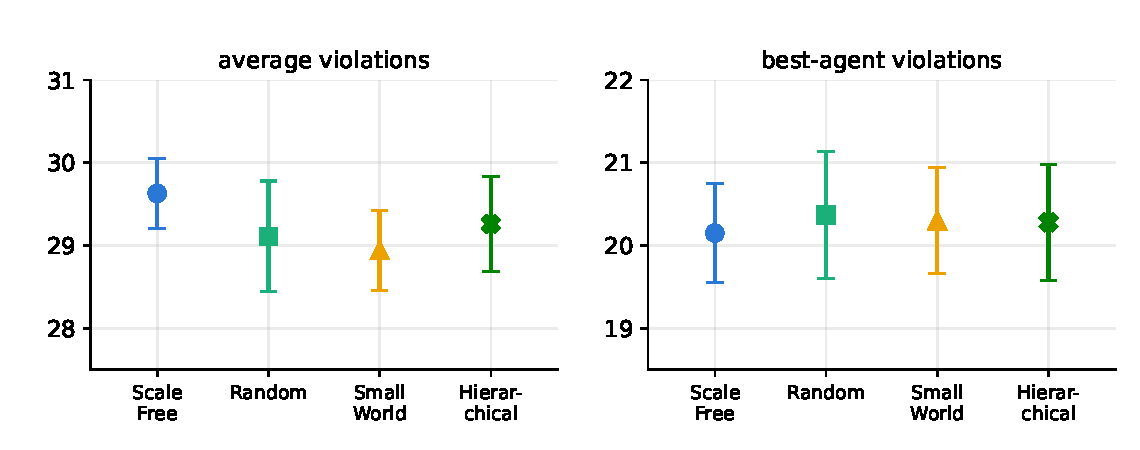
\includegraphics[width=0.8\linewidth]{figs/h1_topology.pdf}
\caption{Long-run average (left) and best-agent (right) violations by topology. Points are seed means $\pm$ 1 s.d.\ over ten seeds.}
\label{fig:h1}
\end{figure}

\subsubsection{Position and performance}

Within every network, agents with higher in-degree do better (Table~\ref{tab:h2}). The Spearman correlation between in-degree and long-run violations lies between $-0.49$ and $-0.62$, and it is negative in all 40 runs. The eight agents with the highest in-degree outperform the eight with the lowest by 3.2 to 4.8 violations. In the scale-free network the best performer sits, on average, at the 95th percentile of in-degree.

\begin{table}[H]
\centering
\caption{Position and performance by topology (10 seeds; mean $\pm$ 1 s.d.). $\rho$: Spearman correlation between in-degree and long-run violations. Gap: mean violations of the eight agents with the highest in-degree minus the eight with the lowest, so a negative gap means the better-connected do better. Last column: mean in-degree percentile of the best performer.}
\label{tab:h2}
\small
\begin{tabular}{@{}lccc@{}}
\toprule
Network & $\rho(k, V)$ & Gap (top 8 minus bottom 8) & Best-agent percentile \\
\midrule
Scale free  & $-0.61 \pm 0.09$ & $-4.8 \pm 1.1$ & 95\% \\
Random      & $-0.57 \pm 0.09$ & $-3.6 \pm 0.7$ & 88\% \\
Small world & $-0.49 \pm 0.10$ & $-3.2 \pm 0.7$ & 71\% \\
Layered     & $-0.62 \pm 0.08$ & $-4.3 \pm 0.9$ & 88\% \\
\bottomrule
\end{tabular}
\end{table}

Pooling the agents shows that the relation is the same in every topology (Fig.~\ref{fig:curve}). Violations fall from about 31 at in-degree 0-1 to about 27.7 at in-degree 8, and to about 25 on the hub tail (in-degree 19 or more) that only the scale-free network has. Designed networks with uniform in-degree distributions extend the mean in-degree from about 4 to about 50 (Fig.~\ref{fig:multinet}). Within each network violations fall with in-degree, while the network averages barely move: a line fitted through them has slope $-0.002$ violations per unit of mean in-degree ($r = -0.11$). Plotted against intake $k/\langle k\rangle$ in place of in-degree, the curves from sparse and dense networks collapse onto one (Fig.~\ref{fig:collapse}).

\begin{figure}[H]
\centering
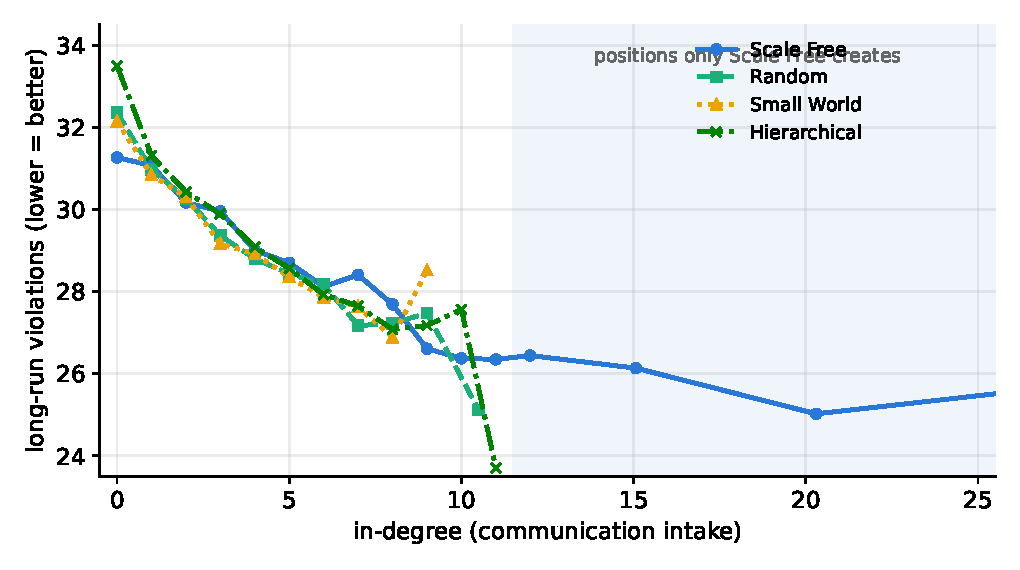
\includegraphics[width=0.68\linewidth]{figs/curve_lbt.pdf}
\caption{Per-agent long-run violations against in-degree, pooled over ten seeds per topology (bins with at least five agents). The four networks trace the same declining curve. The shaded region marks in-degrees that only the scale-free network produces.}
\label{fig:curve}
\end{figure}

\begin{figure}[H]
\centering
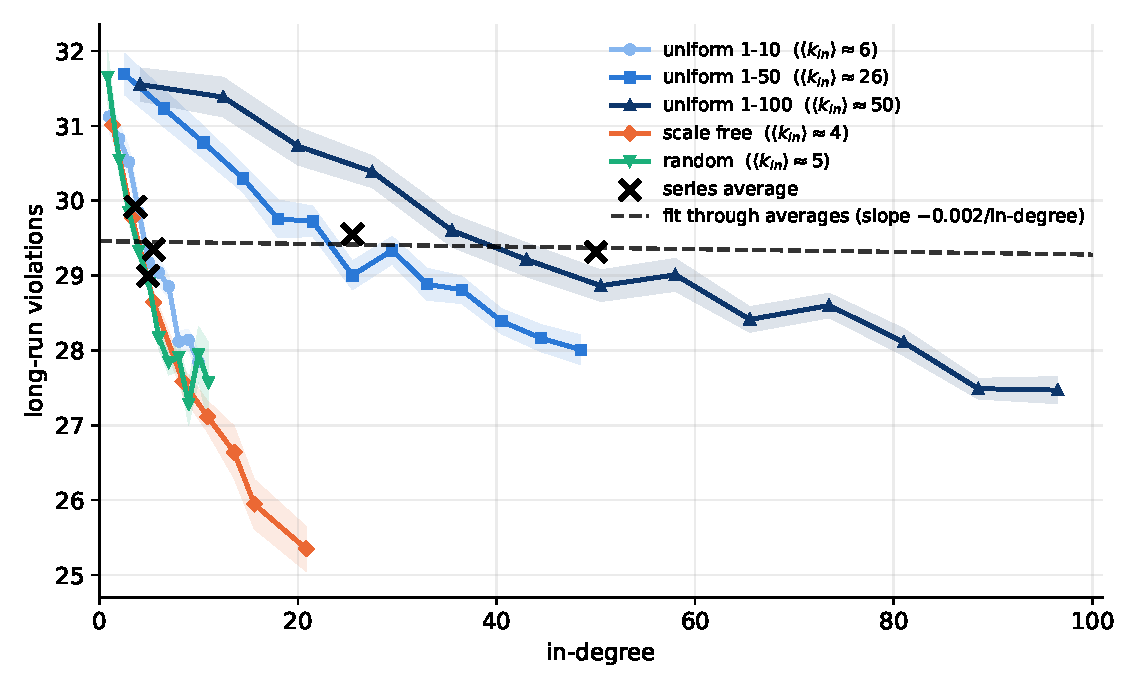
\includegraphics[width=0.78\linewidth]{figs/curve_multinet_degree.pdf}
\caption{Long-run violations against in-degree for five networks with mean in-degree from about 4 to about 50 (at least eight seeds each; bands $\pm 1$ s.e.m.). Crosses mark network averages, and the dashed line is a least-squares fit through them (slope $-0.002$, $r = -0.11$).}
\label{fig:multinet}
\end{figure}

\begin{figure}[H]
\centering
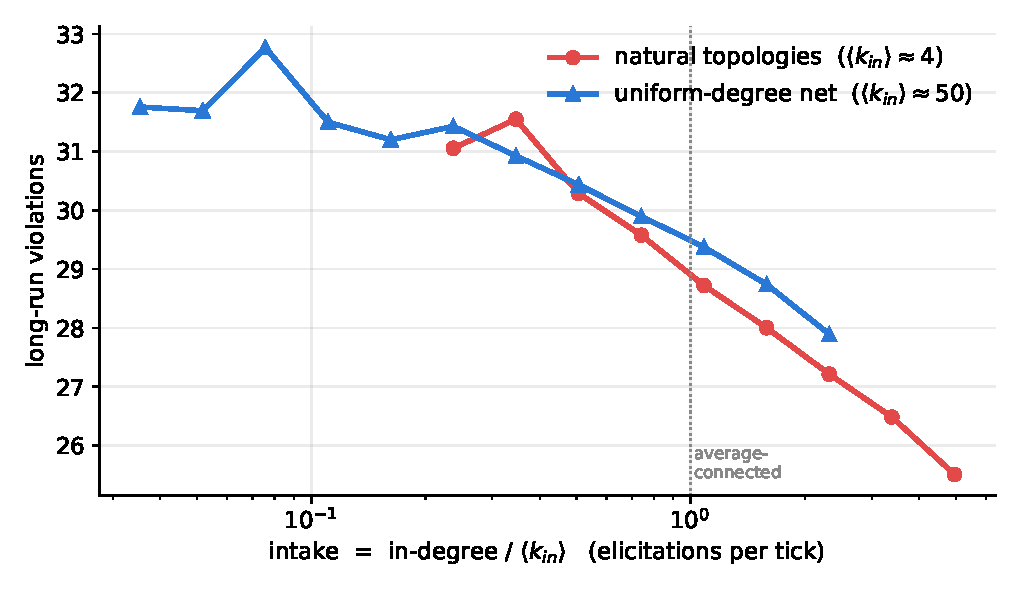
\includegraphics[width=0.6\linewidth]{figs/curve_intake_collapse.pdf}
\caption{Long-run violations against intake $k/\langle k\rangle$ (log scale) for networks with mean in-degree about 4 and about 50. \todo{overlay the theoretical curve when available}}
\label{fig:collapse}
\end{figure}

\subsubsection{Short-run dynamics}

\todo{New runs under the default model. (a) The approach to the long run from empty belief stores, by topology. (b) Recovery after a shock in which a large share of $\mathcal{C}$ is replaced at once, which defines a short run that does not depend on the artificial empty start. Candidate measures: time for $\bar V$ to come within a set margin of its long-run level; stale share after the shock; how far a single fresh clause has spread after $t$ periods.}

\begin{figure}[H]
\centering
\placeholder{$\bar V$ (and the stale share) against time after a shock, by topology.}
\caption{Short-run dynamics. \todo{produce}}
\label{fig:short}
\end{figure}

\subsection{Solving the model: short run}

\todo{AZ, JGR: develop; everything in this subsection is a proposal to be checked against Fig.~\ref{fig:short}.}

Before retirements and the capacity limit start to matter, the live knowledge of a degree-$k$ agent grows through discovery and communication. Writing $T_k$ for the agent's live positive beliefs and $B_k$ for the size of its store, both as fractions of $M$, and $W_k$ for the live clauses it wrongly disbelieves,
\[
\dot T_k \;=\; \underbrace{\frac{1 - T_k - W_k}{2\,(|\mathcal{U}| - B_k M)}}_{\text{discovery}}
\;+\; \underbrace{\frac{\lambda_k\, \pi_T}{M}}_{\text{communication}}
\;-\; \underbrace{\frac{T_k}{M\tau}}_{\text{retirement}} \;+\; \cdots,
\]
where $\pi_T$ is the probability that a received belief is a live clause the receiver lacked, and the dots stand for sign flips and eviction (Supplementary Note 1). Discovery and retirement do not depend on position. Intake enters only through the communication term. \todo{closure for $\pi_T$: the audit showed it cannot be read off the composition of agents' stores}

How fast a single new clause spreads is where structure comes in. Let $I_i(t)$ be the probability that agent $i$ holds a clause that one agent has just discovered. While few agents hold it, a holder $j$ passes it to each out-neighbour with probability $s\,q$ per period, where $q$ is the probability that the clause is still $j$'s freshest disagreement with that neighbour. Linearising,
\[
\dot{\mathbf{I}} = s\,q\,A^{\top}\mathbf{I}
\quad\Longrightarrow\quad
\mathbf{I}(t) \sim e^{g t},
\qquad
g = s\,q\,\Lambda_{\max}(A) = q\,\frac{\Lambda_{\max}(A)}{\langle k\rangle},
\]
where $A_{ji} = 1$ if $j \to i$ and $\Lambda_{\max}$ is the largest eigenvalue of $A$. Normalisation fixes mean intake, but it leaves $\Lambda_{\max}/\langle k\rangle$ free. Without degree-degree correlations, $\Lambda_{\max} \approx \langle k_{\mathrm{in}} k_{\mathrm{out}}\rangle / \langle k\rangle$ \todo{cite Restrepo, Ott \& Hunt (2007), Phys.\ Rev.\ E, on approximating the largest eigenvalue; add to bib}, so
\[
\frac{\Lambda_{\max}}{\langle k\rangle} \;\approx\; \frac{\langle k_{\mathrm{in}} k_{\mathrm{out}}\rangle}{\langle k\rangle^{2}} \;=\; 1 + \frac{\operatorname{cov}(k_{\mathrm{in}}, k_{\mathrm{out}})}{\langle k\rangle^{2}}.
\]
Structure therefore enters the early growth rate through one number, the covariance between an agent's in-degree and its out-degree. It is close to zero in the random and layered networks, positive in the scale-free network, where hubs both hear and speak a lot, and negative in the small-world network. The prediction is that new information spreads fastest in the scale-free network and slowest in the small-world one. In this approximation the time for a clause to reach a given share of agents grows with network size only as $\ln N / g$. \todo{compute $\Lambda_{\max}$ for the generated networks; characterise $q$ under recency; test against Fig.~\ref{fig:short}}

\subsection{Solving the model: long run}

\todo{AZ, JGR: turn the three steps below into stated propositions.}

The long-run results follow from three steps. The first is the intake identity~\eqref{eq:intake}: $\lambda_i = k_i/\langle k\rangle$, with mean exactly 1 on every network.

The second concerns the assignment. Let $p_k$ be the share of ones in a degree-$k$ agent's assignment and $a_k$ the rate at which it acquires positive beliefs. In degree-resolved mean field,
\[
\dot p_k = \frac{2\,a_k}{K}\Bigl[(1 - p_k)\Pr(Z > 0) - p_k\Pr(Z < 0)\Bigr],
\qquad Z = A_1 + X_0 - X_1,
\]
where, for the variable being examined, $A_1$ counts the agent's positive \textsc{and} beliefs whose other variable is 1, and $X_0$ and $X_1$ count its positive \textsc{xor} beliefs whose other variable is 0 and 1. The repair rule accepts a flip from 0 to 1 exactly when $Z > 0$ and from 1 to 0 exactly when $Z < 0$. We checked this against 505,000 logged repair decisions and found no mismatch. The factor $2/K$ is pure counting: each acquisition triggers two examinations, and each accepted flip moves $p_k$ by $1/K$. At a steady state
\[
p_k^{*} = \frac{r_k}{1 + r_k}, \qquad r_k = \frac{\Pr(Z > 0)}{\Pr(Z < 0)}.
\]
The acquisition rate $a_k$, which is where intake enters directly, cancels. Position acts on the assignment only through the composition of the agent's beliefs, which sets the distribution of $Z$. \todo{The standard closure for $\Pr(Z \gtrless 0)$ treats $X_0$ and $X_1$ as independent Poisson counts. It gives $r = 1.81$ and $p^{*} = 0.64$, where the simulation gives $r = 2.33$ and $p^{*} = 0.70$ (measured at $\tau = 10$). Fix, or state as a limitation.}

The third step turns the universal curve into a statement about structure. Suppose, as Fig.~\ref{fig:collapse} indicates, that an agent's long-run violations depend on its position only through intake, $V_i \approx V(\lambda_i)$, with the same function $V$ on every network. Expanding around the mean intake $\lambda = 1$,
\[
\bar V \;\approx\; V(1) + \tfrac{1}{2}\,V''(1)\operatorname{Var}(\lambda),
\qquad
\operatorname{sd}(V) \;\approx\; \lvert V'(1)\rvert\,\operatorname{sd}(\lambda).
\]
Structure moves average performance only at second order, through the curvature of $V$ times the dispersion of intake. It moves the dispersion of performance at first order. The simulated curve is convex: violations fall by about 0.47 per extra link between in-degree 1 and 8, and by roughly half that between 8 and 19. The expansion therefore predicts that the network with the most dispersed in-degree does slightly worse on average, and the scale-free network does. \todo{check the size: predict each network's $\bar V$ from the pooled curve and its in-degree distribution. The expansion is poor near $\lambda = 0$, where agents with no in-links sit on the steep part of the curve.}

What remains is to derive $V(\lambda)$ itself: why violations fall with intake, and how fast. The mechanism runs through the stocks of live and stale beliefs. More intake brings more live clauses and, under the recency rule, more corrections of stale ones. Supplementary Note 1 sets out a compartment model of live, stale and negative beliefs by degree class, and an age-structured model of the contest that follows each retirement. In the latter the recency rule enters through a single asymmetry parameter $\kappa$, the net share by which corrections outnumber re-infections, measured at about 3\% of gross flows early in a run and 17\% late. \todo{$\tau = 10$ measurements; redo at $\tau = 1$. Missing piece: a map from belief composition $(T_k, S_k)$ to violations $V_k$.}


%======================================================================
\section{Discussion}\label{sec:discussion}
%======================================================================

\todo{short-run finding, once the runs are in.} Once the communication rate is equalised, long-run average performance does not depend on network structure, across four standard topologies and a thirteen-fold range of density. Individual performance does depend on position. It depends on it through intake, along a curve that is the same in every network, so the shape of the network decides who is well informed and leaves the average almost untouched.

For organisational design this recasts centralisation as a way of choosing who is well informed. In a network with homogeneous degrees, the best-informed member owes the position to small random differences. In a centralised network the high-intake seats are designed, and whoever occupies them outperforms the periphery by several violations; in our scale-free runs the best performer sits at the 95th percentile of in-degree. That is useful when decision rights or attention are scarce and have to be concentrated. The average hides the price. The arithmetic that gives the hubs their advantage leaves a large periphery with little intake, which is why the scale-free network does slightly worse overall. \todo{connect to \textcite{simon1962architecture}, \textcite{bolton1994firm} and \textcite{lazer2007network}}

\todo{depends on the short-run results.} If structure matters mainly in the transient, it matters most when transients are frequent: after a merger, a regulatory overhaul or a technology shock, when much of what an organisation knows becomes wrong at once. In that phase the speed at which corrections travel, which the short-run argument ties to the covariance of in- and out-degree, may matter more than where the organisation eventually settles.

Several extensions follow. Agents here are identical and follow fixed rules. Behavioural heterogeneity, such as differences in testing capacity or in willingness to pass on negative results, would let position and ability interact. Links and the communication rate are fixed from outside, whereas in real organisations people choose whom to consult and how often, which could compound the advantage of central positions. Two limitations point the same way. Our layered network has layers but no hubs, so it behaves like the random one, and a generator with real asymmetry between levels is needed to speak to hierarchy in the organisational sense. The mean-field treatment of the repair step also remains approximate. \todo{trim}


%======================================================================
\section*{Data availability}
Simulation outputs underlying the figures, and the scripts that produce them, will be deposited in a public archive at submission. \todo{Zenodo DOI}

\section*{Code availability}
The model, analysis scripts and an interactive browser animation are available at \url{https://github.com/atiyabzafar/architecturesofproblemsolving}. The animation also runs at \url{https://fausto.ge/problem-solving/}. \todo{confirm repository visibility; release tag}

\section*{Author contributions}
\todo{draft} FG conceived the model extensions, ran the simulations and analyses and wrote the manuscript. AZ and JGR developed the mean-field theory, and AZ co-developed the model implementation. JGR supervised the analytical work. PA built the interactive application. All authors discussed the results and revised the manuscript.

\section*{Competing interests}
The authors declare no competing interests.

\section*{Acknowledgements}
The authors thank the faculty of the Complexity Global School 2025 (Santa Fe Institute and Universidad de los Andes, Bogot\'a). \todo{funding statement goes here; the journal does not allow a separate one}

\printbibliography


%======================================================================
\clearpage
\section*{Supplementary Information}
%======================================================================

\subsection*{Supplementary Note 1: full theory derivations}

\todo{AZ, JGR, FG. Planned contents below; most of the material exists in the August 2026 audit notes, derived and validated at $\tau = 10$.}

The note will start from a degree-resolved compartment model. Each agent's store is split into live positive beliefs $T_k$, stale positive beliefs $S_k$ and negative beliefs $N_k$, with wrong negatives $W_k$ tracked as a subset of $N_k$, all as fractions of $M$. Communication is split into additions, which use a memory slot, and sign flips, which do not; only additions can force an eviction. Adding the equations shows that the store grows only through discovery and additions and shrinks only through eviction, which gives a check on the bookkeeping.

The second part is the age-structured model of what happens after a retirement. For a clause retired $a$ periods ago, $h(a)$ is the share of agents still believing it and $n(a)$ the share disbelieving it, starting from $h(0) = T$ and $n(0) = 0$. Testing moves agents from $h$ to $n$ at rate $\theta = 1/(2\bar B M)$; communication moves them both ways, and the recency rule sets the net direction through $\kappa$. Summing over cohorts gives $S$ and the dead-clause part of $N$.

The third part covers the repair step: the derivation of the acceptance rules and of the factor $2/K$, the closure for $\Pr(Z \gtrless 0)$, and its known errors. The fourth compares every flow in the model with instrumented simulations. \todo{redo the validation at $\tau = 1$}

\end{document}
